\documentclass{article}
\usepackage{tikz}
\usepackage{amsmath}
\usetikzlibrary{shapes.geometric, positioning}

\begin{document}

\section*{Asignacion del tablero}

Sean \( r_1, \ldots, r_m \) y \( c_1, \ldots, c_n \) números naturales. Se quiere asignar los valores de las celdas de una matriz de \( m \times n \) con números naturales de forma tal que la i-ésima fila sume \( r_i \) y la i-ésima columna sume \( c_i \).

\subsection*{a) Modelar el problema de asignación como un problema de flujo}

Pensamos en el siguiente grafo: el tablero nos define dos conjuntos bipartitos, el valor de una columna \( c_i \) solo depende del valor de las filas \( f_1, f_2, \ldots, f_n \) en la posición de la columna. Eso nos define una relación entre las particiones. Podemos modelar estas relaciones como un grafo, teniendo a cada \( c_i \) y \( f_j \) como vértices en él, siendo las aristas las relaciones correspondientes. Observemos que cada columna se relaciona con todas las filas y viceversa. Luego podemos establecer nuestra fuente \( s \) y nuestro sumidero \( t \). Las capacidades entre la fuente y las columnas son iguales a \( c_i \) para cada columna, y las de las filas al sumidero son \( r_j \). Las capacidades de las aristas intermedias son infinitas (ya están acotadas por las capacidades que salen de la fuente).

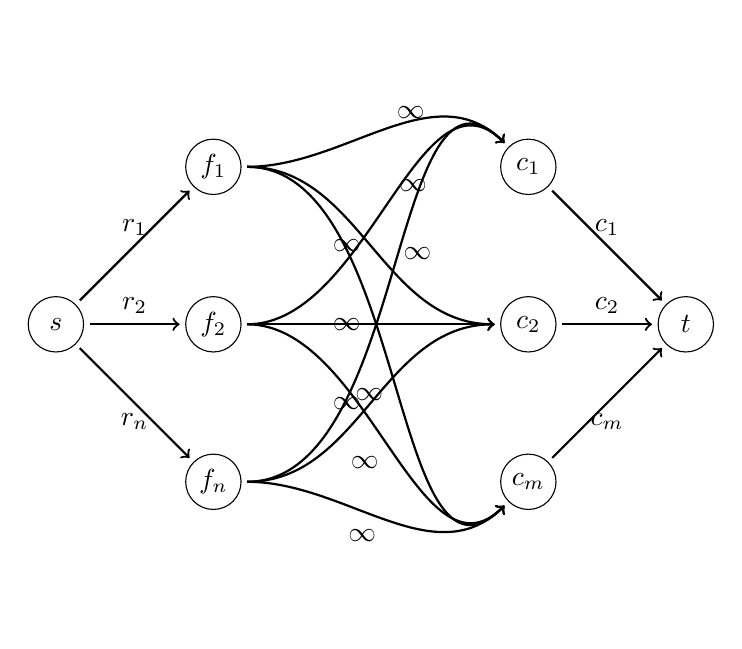
\begin{tikzpicture}[
    vertex/.style={circle, draw, minimum size=20pt, inner sep=0pt},
    edge/.style={->, thick, shorten >=2pt, shorten <=2pt}
]
    % Vertices representing rows and columns
    \node[vertex] (f1) at (0,2) {$f_1$};
    \node[vertex] (f2) at (0,0) {$f_2$};
    \node[vertex] (fn) at (0,-2) {$f_n$};
    
    \node[vertex] (c1) at (4,2) {$c_1$};
    \node[vertex] (c2) at (4,0) {$c_2$};
    \node[vertex] (cm) at (4,-2) {$c_m$};
    
    % Source and sink
    \node[vertex] (source) at (-2,0) {$s$};
    \node[vertex] (sink) at (6,0) {$t$};
    
    % Edges
    \draw[edge] (source) to node[above] {$r_1$} (f1);
    \draw[edge] (source) to node[above] {$r_2$} (f2);
    \draw[edge] (source) to node[below] {$r_n$} (fn);
    
    \draw[edge] (c1) to node[above] {$c_1$} (sink);
    \draw[edge] (c2) to node[above] {$c_2$} (sink);
    \draw[edge] (cm) to node[below] {$c_m$} (sink);
    
    % Connections between rows and columns
    \draw[edge] (f1) to[out=0,in=135] node[midway, above right] {$\infty$} (c1);
    \draw[edge] (f1) to[out=0,in=180] node[midway, left] {$\infty$} (c2);
    \draw[edge] (f1) to[out=0,in=225] node[midway, below left] {$\infty$} (cm);
    
    \draw[edge] (f2) to[out=0,in=135] node[midway, above right] {$\infty$} (c1);
    \draw[edge] (f2) to[out=0,in=180] node[midway, left] {$\infty$} (c2);
    \draw[edge] (f2) to[out=0,in=225] node[midway, below left] {$\infty$} (cm);
    
    \draw[edge] (fn) to[out=0,in=135] node[midway, above right] {$\infty$} (c1);
    \draw[edge] (fn) to[out=0,in=180] node[midway, left] {$\infty$} (c2);
    \draw[edge] (fn) to[out=0,in=225] node[midway, below left] {$\infty$} (cm);
\end{tikzpicture}

Luego de obtener algun flujo máximo, podemos hacer las siguientes conclusiones:
\begin{itemize}
    \item La asignacion pedida es posible $\iff$ las aristas de salida de la fuente y de entrada al sumidero están saturadas, ya que quiere decir que nuestra suma de valores es posible.
    
    \item Cada unidad de flujo de una arista $(f_i,c_j)$ corresponde al valor que le daremos en el tablero a la posición $(i,j)$ correspondiente (ya que la intersección entre una fila y una columna es una sola casilla).
\end{itemize}

Complejidad:

Podemos calcular la cantidad de aristas en nuestro grafo. Si tenemos $n$ columnas y $m$ filas, sabiendo que todos están conectados con todos, además de que todos están conectados a la fuente o el sumidero respectivamente, tenemos que
\[
|E| := \binom{n+m}{2} + n + m = \frac{n^2 + 2nm + m^2 - n - m}{2} + n + m = \frac{n^2 + m^2}{2} + nm - \frac{n + m}{2}
\]
\[
|V| := n + m + 2
\]

Entonces si la complejidad de Edmonds-Karp es de \\ 
$O(\min(|V||E|^2, |V|F)) = O\left(\min \left( (n^2 + m^2 + nm)^2 \cdot (n+m), (n+m) \cdot F \right)\right)$.


\end{document}
